\chapter{LLM-Inferred Substitute and Complement Signals for Recommendation}~\label{chpt:erlsc}

\section{Introduction}
Substitution and complementarity are fundamental item-item relations for understanding user intent in recommendation systems~\cite{subcom22, subcom23}. Substitutes represent alternatives that satisfy the same user need, while complements capture items that are jointly consumed within a coherent usage context. 
For example, an on-ear headphone and an over-ear headphone serve similar listening purposes and can be regarded as substitutes, whereas adapters are typically complementary accessories that support headphone usage in cellphones. Recommending such substitute or complementary items to an on-ear headphone buyer can improve user satisfaction by offering meaningful alternatives. 
However, ground-truth annotations of substitute and complementary relations are rarely available in public datasets~\cite{dataset:amazon, xmarket}, and obtaining reliable annotations through manual labeling is costly and time-consuming. Consequently, prior work~\cite{sclabel20chen, sclabel20liu, sclabel20xu} typically relies on co-view or co-purchase signals as weak supervision. However, directly treating these signals as substitutes or complements implicitly assumes that behavioral co-occurrence aligns with real-world item relations, an assumption that frequently fails in practice~\cite{notrealsc22tong, notrealsc23ye, notrealsc24kai}. Many co-occurring item pairs are neither substitutes nor complements, but arise from incidental browsing or exploratory interactions. On e-commerce platforms, users often interact with multiple unrelated items within a short time window, resulting in co-occurrence records that are incidental rather than semantically meaningful.

Ideally, a solution should possess human-like world knowledge to distinguish true substitute and complementary relations from incidental co-occurrences, while avoiding the high cost and inefficiency of large-scale manual annotation. Recent advances in LLMs offer a promising way to address these challenges, as they encode rich world knowledge about usage contexts acquired from large-scale text corpora. This knowledge enables LLMs to move beyond surface-level co-occurrence patterns and reason about the functional roles items play in real-world scenarios. 
Benefiting from this semantic reasoning capability, LLMs have been applied for labeling substitute and complementary relations in previous works~\cite{llmlabel23papso, llmlabel25Hosseini}.

To effectively harness the world knowledge of LLMs on substitutes and complements for recommendation, we propose ERLSC, which leverages LLMs to distinguish true substitute and complementary relations from noisy co-occurring item relations for enhanced recommendation. We adopt a hypergraph formulation because co-view and co-purchase signals naturally induce item groups rather than isolated item pairs, and hyperedges provide a principled way to model such higher-order co-occurrence relations. By assigning weights to hyperedges via an LLM, ERLSC can selectively emphasize item groups that exhibit coherent substitute or complement semantics while down-weighting irrelevant co-occurrences.
To incorporate LLM-derived semantic signals into this structure, we design an LLM-Guided Hypergraph Convolution (LGHC) layer to initialize and update hyperedge weights in an item-item hypergraph. Specifically, we first construct hyperedges by connecting frequently co-occurring items in user interaction logs. We then query LLMs to assess how many item pairs within each hyperedge reflect true substitute or complementary relations. The resulting relation composition is used to initialize hyperedge weights, which are further refined during training through weight modulation.
The key contributions are:
\begin{itemize}[left=0pt]
    \item We propose a novel recommendation framework ERLSC. As far as we know, this is the first work enhancing recommendation via LLM-inferred substitute and complement signals.
    \item We introduce an LGHC layer that seamlessly integrates LLM-based relation assessment into hypergraph modeling by initializing and adaptively updating hyperedge weights.
    \item We conduct extensive experiments on three public datasets to demonstrate the effectiveness of ERLSC, and perform ablation studies to verify the contribution of each component.
\end{itemize}

\section{Preliminaries}\label{sec_erlsc:pre}

\subsection{Problem Formulation} 
Let $\mathcal{I}$ and $\mathcal{U}$ denote the complete item pool and the set of users in the dataset, respectively. Given the user-item interactions as edges $E_{\mathcal{U},\mathcal{I}}$, a user-item graph is defined as $\textit{G}=(V,E)$ where $V = \mathcal{U} \cup \mathcal{I}$. Each item $i \in \mathcal{I}$ is accompanied by its corresponding textual description $\text{desc}(i)$. In addition, items that appear in the same co-view or co-purchase group are connected by a hyperedge. 
An incidence matrix $\mathbf{H}\in\{0,1\}^{|\mathcal{I}|\times|\mathcal{E}|}$ is used to represent the connections between items $\mathcal{I}$ and hyperedges $\mathcal{E}$ in the item-item hypergraph. 
Given a user $u \in \mathcal{U}$, the recommendation task is to predict a ranked list of items $\{i_1, i_2, \dots, i_m\}$ that the user has not interacted with in the graph $\textit{G}$.

\subsection{Collaborative Filtering}
To learn representations of users and items from interactions, we apply collaborative filtering (CF) on the user-item graph $\textit{G}$. CF captures collaborative signals by modeling historical user-item interactions, which are essential for inferring user preferences and item relevance in recommendation. 
We maintain an embedding layer $\mathbf{E}\in \mathbb{R}^{d\times(|\mathcal{U}|+|\mathcal{I}|)}$, where $d$ denotes the embedding dimension. Through CF, we obtain user embeddings $\mathbf{E}'_{\mathbf{u}}$ and item embeddings $\mathbf{E}'_{\mathbf{i}}$, which encode collaborative patterns from the interaction graph. The learned user embeddings are subsequently used to perform personalized ranking over candidate items in the recommendation task.
In this work, we adopt a one-layer LightGCN~\cite{LightGCN} as the underlying graph-based CF model due to its simplicity and effectiveness. 

\section{Proposed Framework: ERLSC}\label{sec_erlsc:model}

\begin{figure*}[]
    \centering
    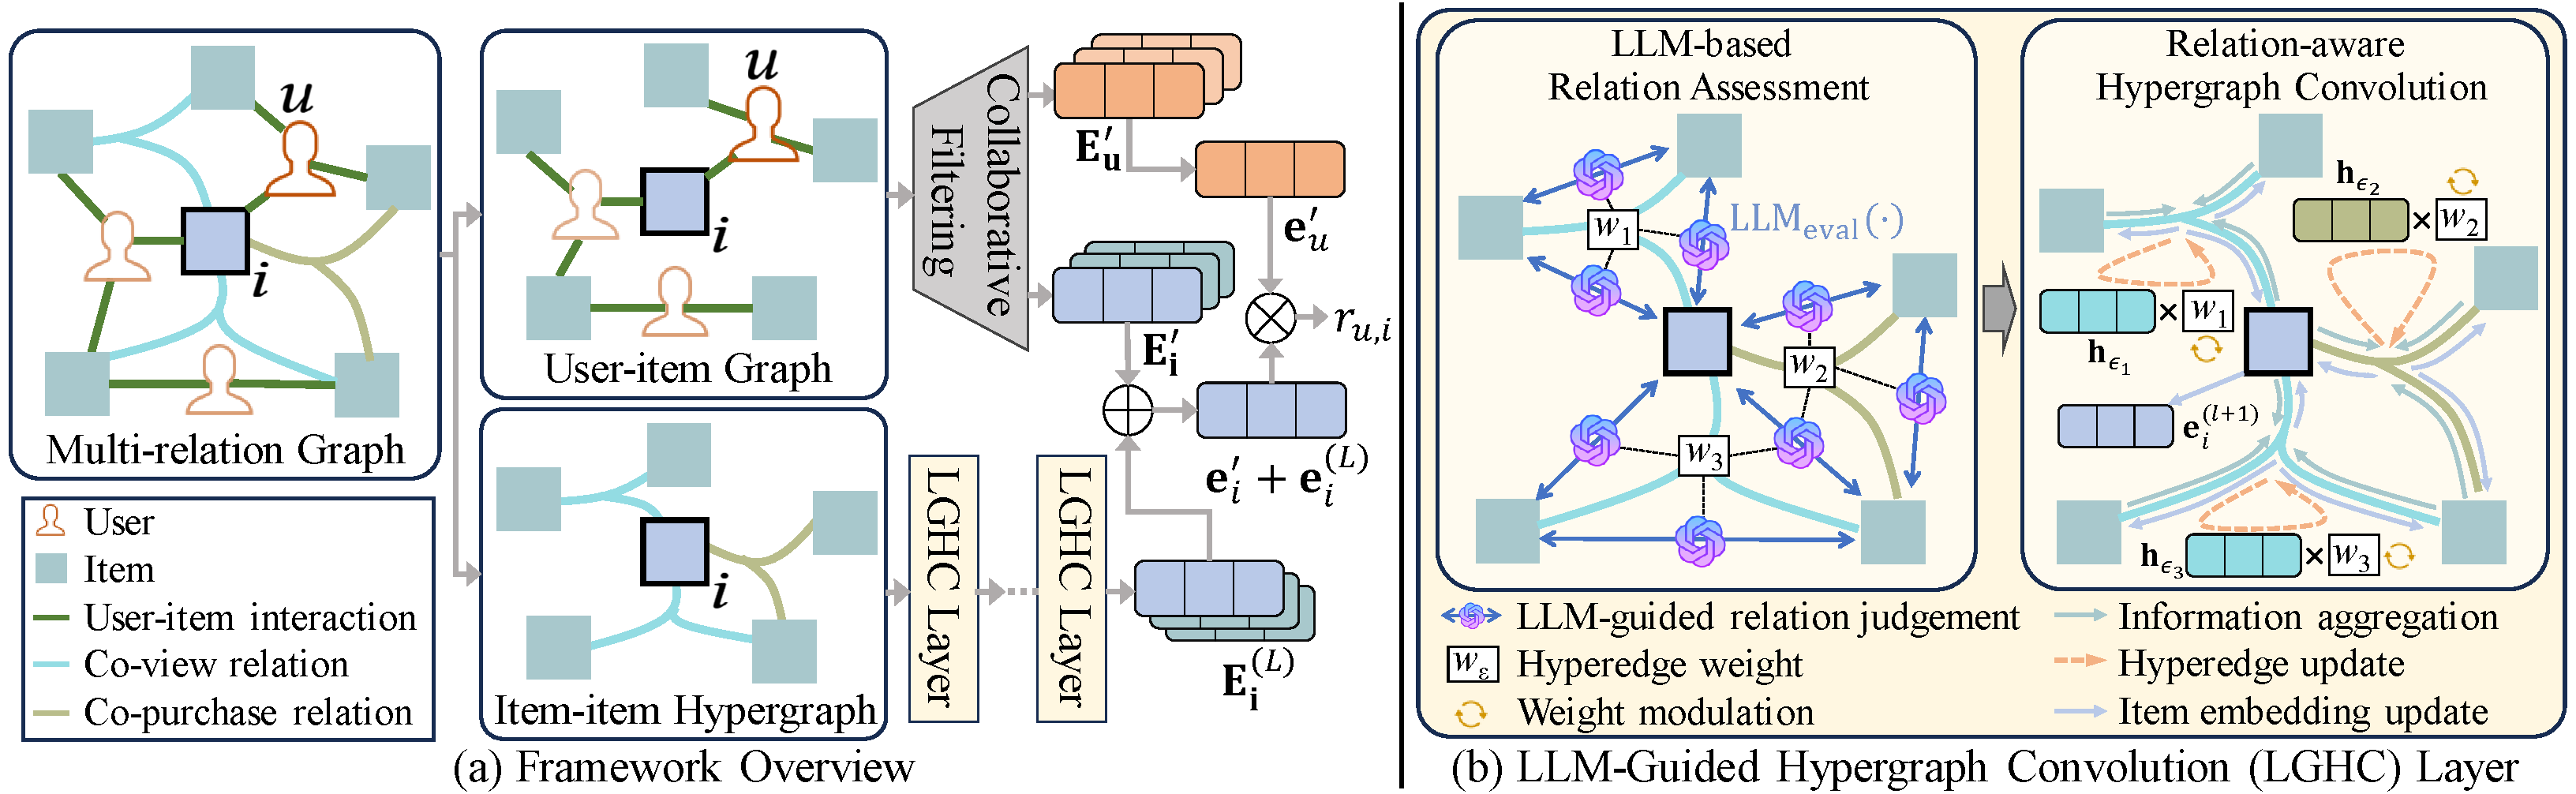
\includegraphics[scale=0.29]{sections/5_ERLSC/figures/framework.pdf}
    \caption{The framework of ERLSC and the proposed LGHC layer.}
    \label{fig:framework}
\end{figure*}

\subsection{LLM-based Relation Assessment}
The overall architecture of ERLSC is illustrated in Figure~\ref{fig:framework}. Beyond the collaborative signals captured by CF, propagating information over item–item hypergraphs is essential for modeling the semantic and functional relationships implicit in item co-occurrence. In particular, co-view and co-purchase relations often reflect shared functionality or joint usage patterns that cannot be fully captured by user–item interactions alone. To assess the reliability of each hyperedge in representing such relations, as the first component of the proposed LGHC layer, we leverage LLMs to evaluate its semantic coherence based on LLMs' world knowledge.

Since substitute and complementary relations are more reliably identified at the pairwise level than at the group level, we first query the LLM to assess pairwise relations within each co-occurrence group. Specifically, given a hyperedge $\epsilon$ that connects a group of items $\mathcal{N}_{\epsilon}$, we enumerate all unordered item–item pairs $\mathcal{P}(\mathcal{N}_\epsilon) = \{ (i_j, i_k) \mid i_j, i_k \in \mathcal{N}_\epsilon,\; j < k \}$, and compute the number of item pairs that exhibit substitute or complementary relations as follows:
\begin{equation}\label{eq:gen_prof}
        y^{t}_\epsilon = \sum_{(i, i')\in\mathcal{P}(\mathcal{N}_\epsilon) }\text{LLM}_\text{eval}(t,\text{desc}(i),\text{desc}(i'))
\end{equation}
where $t \in {\text{sub}, \text{com}}$ denotes the relation type being queried, corresponding to substitute or complementary relations, respectively. The function $\text{LLM}_{\text{eval}}(\cdot)$ returns a binary outcome indicating whether the item pair $(i, i')$ exhibits the specified relation. Accordingly, $y_t$ represents the total number of substitute or complement item pairs within the hyperedge.

We then initialize the hyperedge weight based on the proportion of relation-consistent pairs within the group. Specifically, the weight of hyperedge $\epsilon$ is defined as $w_\epsilon = \frac{y^{\text{sub}}_\epsilon+y^{\text{com}}_\epsilon}{|\mathcal{P}(\mathcal{N}_\epsilon)|}$. A larger value of $w_\epsilon$ indicates that a higher fraction of item pairs exhibit either substitute or complementary relations, suggesting that the hyperedge corresponds to a semantically coherent and functionally meaningful co-occurrence pattern. In contrast, a smaller value implies that most item pairs lack clear semantic relations, indicating that the hyperedge is likely noisy or less informative.

\subsection{Relation-aware Hypergraph Convolution}
To incorporate LLM world knowledge as prior semantic guidance and to adaptively refine hyperedge importance during training, we design a relation-aware hypergraph convolution module consisting of three sequential components: information aggregation, hyperedge update, and item embedding update.

\subsubsection{Information Aggregation}
We first construct a representation for each hyperedge by aggregating the embeddings of all items incident to it: 
% Specifically, the embedding of hyperedge $\epsilon$ at the $l$-th layer is computed as
\begin{equation}
    \mathbf{h}_\epsilon^{(l)} = \frac{1}{|\mathcal{N}_\epsilon|} \sum_{i \in \mathcal{N}_\epsilon} \mathbf{e}_{i}^{(l)},
\end{equation}
where $\mathbf{h}_\epsilon^{(l)}$ denotes the embedding of hyperedge $\epsilon$ and $\mathbf{e}_{i}^{(l)}$ is the embedding of each connected item. We adopt mean pooling as aggregation method to summarize information from item nodes.

\subsubsection{Hyperedge Update}
To enable the model to exploit the LLM-initialized hyperedge weights while allowing adaptive refinement during training, we perform weight modulation based on hyperedge-level features. Each hyperedge $\epsilon$ is associated with a feature vector $\mathbf{x}_\epsilon$ that captures both structural and semantic characteristics, including:
the hyperedge degree, the average and maximum degrees of its connected item nodes, $y^\text{sub}_\epsilon$, $y^\text{com}_\epsilon$, $\lvert y^\text{sub}_\epsilon - y^\text{com}_\epsilon \rvert$, and $\lvert \mathcal{P}(\mathcal{N}_\epsilon) \rvert$.
These features are fed into a two-layer multilayer perceptron (MLP) to generate a modulation factor for the hyperedge weight. The reweighted hyperedge embedding is then computed as
\begin{equation}\label{eq:edge_update}
    \mathbf{q}_\epsilon^{(l)} = f_\text{MLP}(\mathbf{x}_\epsilon) \cdot w_\epsilon \cdot \mathbf{h}_\epsilon^{(l)},
\end{equation}
where $w_\epsilon$ is the LLM-initialized hyperedge weight, $f_\text{MLP}(\cdot)$ denotes the weight-modulation MLP, and $\mathbf{q}_\epsilon^{(l)}$ represents the final reweighted embedding of hyperedge $\epsilon$ at layer $l$. This design allows the model to jointly leverage prior semantic reliability from the LLM and task-specific structural cues learned during training.

\subsubsection{Item Embedding Update}
Finally, we update each item embedding by aggregating the reweighted embeddings of all hyperedges incident to the item. For a target item $i$, the update rule is given by
\begin{equation}\label{eq:item_update}
    \mathbf{e}_i^{(l+1)} = \frac{1}{|\mathcal{N}_i|} \sum_{\epsilon \in \mathcal{N}_i} \mathbf{q}^{(l)}_{\epsilon},
\end{equation}
where $\mathbf{e}_{i}^{(l+1)}$ denotes the updated embedding of item $i$, and $\mathcal{N}_i$ is the set of hyperedges connected to item $i$. Through this operation, each item aggregates information from its surrounding hyperedges, with contributions weighted by both LLM-derived semantic confidence and learned structural relevance.

\subsection{Ranking Prediction}
The final item embedding is obtained by adding CF-based item embedding $\mathbf{e}'_i$ to the updated item embedding $\mathbf{e}^{(L)}_i$ from the last LGHC layer. And we compute the ranking score $r_{u,i}$ of the user-item pair $(u,i)$ by the inner product of user and item embeddings: 
\begin{equation}
r_{u,i} = \mathbf{e}_{u}'\cdot (\mathbf{e}'_{i} + \mathbf{e}^{(L)}_i),
\end{equation}
Then, we adopt the pairwise BPR loss~\cite{BPR} to optimize the ranking prediction:
\begin{equation}
    \mathcal{L}=\sum\limits_{(u,i,i^-)\in \mathcal{D}} -\log\sigma(\hat{r}_{u,i}-\hat{r}_{u,i^-}) + \lambda_\Theta\|\Theta\|^2_2,
\end{equation}
where $\mathcal{D}=\{(u,i,i^-)|i\in \mathcal{I}^{+}_{u}, i^-\in \mathcal{I}\backslash\mathcal{I}^{+}_{u}\}$ is the training data and item set $\mathcal{I}^{+}_{u}$ contains all the items interacted by user $u$. We denote all trainable parameters as $\Theta$, regularized by $\lambda_\Theta$. Adam~\cite{Adam} is chosen as the optimizer.

\section{Experiment}
\subsection{Experiment Settings}
\subsubsection{Datasets}
\begin{table}
  \resizebox{0.6\textwidth}{!}{
  \begin{tabular}{l c c c}
        % \toprule
        \hline
        \hline
        \textbf{Dataset} & Electronics & Office & Home \\
        \hline
        \#Users & 12,828 & 7,528 & 1,534\\

        \#Items & 19,297 & 5,743 & 4,923\\

        \#U-I interactions & 93,788 & 40,330 & 7,810\\
        \#\textit{Bought-together} relations & 2,769 & 1,555 &326 \\
        \#\textit{Compared-with} relations & 5,746 & 706 & 614 \\
        \#\textit{Also-bought} relations & 5,852 &696 & 715 \\
        \#\textit{Also-viewed} relations & 15,288 & 3,838 & 2,819 \\
        % \bottomrule
        \hline
  \end{tabular}}
  \caption{Statistics of datasets for ERLSC.}
  \label{tab_erlsc:datasets}
\end{table}
We conduct experiments on three sub-datasets from the public XMarket dataset~\cite{xmarket}: Electronics, Office, and Home. These categories are chosen because they naturally exhibit abundant substitute and complementary item relations, due to overlapping product functionalities and frequent accessory co-usage. The statistics of the selected datasets are summarized in Table~\ref{tab_erlsc:datasets}. We treat \textit{bought-together} and  \textit{also-bought} relations as co-purchase signals, and \textit{compared-with} and \textit{also-viewed} relations as co-view signals.

\subsubsection{Baselines}
To evaluate the effectiveness of ERLSC, we compare it with six baselines, including four representative CF methods: LightGCN~\cite{LightGCN}, HCCF~\cite{hccf}, SimpleX~\cite{simplex}, and DiffRec~\cite{diffrec}. 
Since the datasets also provide sequential order information in user transaction histories, we further compare our method with sequential recommendation baselines, including SASRecCPR~\cite{sascpr} and FeaRec~\cite{fearec}.
All methods are evaluated under the full-ranking setting, where each test user is ranked against all non-interacted items. We adopt Recall (R@5, R@10) and NDCG (N@5, N@10) as evaluation metrics.
 

\begin{table*}[]
\
\resizebox{\textwidth}{!}{
\begin{tabular}{l|rrrr|rrrr|rrrr}
\hline
\hline
Dataset    & \multicolumn{4}{c|}{Electronics}                                                                                       & \multicolumn{4}{c|}{Office}                                                                                            & \multicolumn{4}{c}{Home}                                                                                           \\ \hline
Metric     & \multicolumn{1}{c}{R@10}     & \multicolumn{1}{c}{R@20}    & \multicolumn{1}{c}{N@10}     & \multicolumn{1}{c|}{N@20}    & \multicolumn{1}{c}{R@10}     & \multicolumn{1}{c}{R@20}    & \multicolumn{1}{c}{N@10}     & \multicolumn{1}{c|}{N@20}   & \multicolumn{1}{c}{R@10}     & \multicolumn{1}{c}{R@20}    & \multicolumn{1}{c}{N@10}     & \multicolumn{1}{c|}{N@20}     \\ \hline
LightGCN   & {\ul 0.0894}                      & 0.0959                      & {\ul 0.0786}                     & 0.0804               & {\ul 0.2489}                     & {\ul 0.2692}                     & 0.2141                     & 0.2195                       & 0.1118                     & 0.1199                      & {\ul 0.0910}                       & 0.0930                       \\
SimpleX       & 0.0860                      & 0.0924                     &0.0779                      & 0.0797                       &0.2444                      & 0.2583                      & 0.2136                     & 0.2174                       & 0.1098                      & 0.1167                    &0.0872                       & 0.0888                      \\
DiffRec  & 0.0743                      & 0.0801                      & 0.0680                      & 0.0696                      & 0.2405                      & 0.2524                      & {\ul 0.2167}                      &0.2199                       & 0.1074                &0.1172                      & 0.0816                      & 0.0838                    \\
SASRecCPR      & 0.0665                      & 0.0961                      & 0.0700                      & 0.0729                       & 0.1925                      & 0.2111               & 0.1966                      & 0.2010                       & 0.1151                     &    0.1235                    & 0.0683                       & 0.0751                   \\
FeaRec  & 0.0704                      & 0.0897                      & 0.0607                      & 0.0656                 & 0.1829                & 0.1963                      & 0.1698                & 0.1739                 
&{\ul 0.1206}                     &{\ul 0.1319}               & 0.0887                 & {\ul 0.0941}                 \\
HCCF & 0.0827                &{\ul 0.1025}                      & 0.0783                     & {\ul 0.0845}                       & 0.2167                      & 0.2624                      & 0.1986                      & {\ul 0.2272}                      & 0.1133                      & 0.1214                      & 0.0839                       & 0.0865                       \\ \hline
ERLSC      & \textbf{0.1232}             & \textbf{0.1337}             & \textbf{0.1034}             & \textbf{0.1062}              & \textbf{0.2816}             & \textbf{0.3045}             & \textbf{0.2404}             & \textbf{0.2467}              & \textbf{0.1325}             & \textbf{0.1423}             & \textbf{0.1131}              & \textbf{0.1157}              \\ \hline
Improv.    & \multicolumn{1}{l}{37.78\%} & \multicolumn{1}{l}{30.45\%} & \multicolumn{1}{l}{31.54\%} & \multicolumn{1}{l|}{25.62\%} & \multicolumn{1}{l}{13.11\%} & \multicolumn{1}{l}{13.10\%} & \multicolumn{1}{l}{10.96\%} & \multicolumn{1}{l|}{8.60\%} & \multicolumn{1}{l}{10.44\%} & \multicolumn{1}{l}{7.84\%} & \multicolumn{1}{l}{24.20\%} & \multicolumn{1}{l}{22.99\%} \\ \hline
\end{tabular}
}\caption{Overall performance comparison of ERLSC with baselines.}\label{tab_erlsc:overall}
\end{table*}

\subsection{Overall Performance}
The overall performance comparison between ERLSC and the baseline methods is reported in Table~\ref{tab_erlsc:overall}. We make the following observations.
First, ERLSC consistently outperforms all baseline methods across all datasets and evaluation metrics. The improvements are particularly pronounced on the Electronics dataset, where rich co-view and co-purchase signals are available. This result demonstrates the effectiveness of incorporating item–item relations to capture functional item groupings.
Second, the hypergraph-based baseline HCCF constructs hyperedges by connecting all items interacted with by the same user. This strategy remains sensitive to sparse user–item interactions, such as Home dataset where user behaviors are less dense. In contrast, ERLSC constructs hyperedges from item co-occurrence relations and further leverages LLM-based semantic assessment to weight these hyperedges, allowing the model to emphasize meaningful substitute and complementary relations while suppressing irrelevant co-occurrences. This design enables ERLSC to achieve robust performance even when behavioral signals are noisy or limited.



\subsection{Ablation Study}
To verify the effectiveness of each component in ERLSC, we conduct ablation studies by comparing it with several variants, as shown in Figure~\ref{fig:ablation}. 
The variant \textit{w/o H} considers only user-item interactions without item–item hypergraph modeling.
The variant \textit{H} replaces the LGHC layer in ERLSC with a hypergraph convolution layer, where all hyperedges have equal weights $w_\epsilon =1$.
The variant \textit{LH} further incorporates LLM-initialized hyperedge weights, but disables weight modulation during training.
From the results, we observe a consistent performance improvement when hypergraph information is introduced. 
Moreover, by incorporating LLM-initialized hyperedge weights, the \textit{LH} variant further improves performance, demonstrating that LLM-based semantic assessment helps identify hyperedges that better reflect substitute and complementary relations. Finally, the best performance of ERLSC on all datasets highlights the importance of dynamically modulating hyperedge weights during training, which allows the model to adaptively refine the influence of each hyperedge based on recommendation objectives. 
Overall, the ablation results confirm that both LLM-guided hyperedge initialization and weight modulation are critical components for achieving optimal performance.


 
\begin{figure}[]
    \begin{subfigure}{0.3\textwidth}
    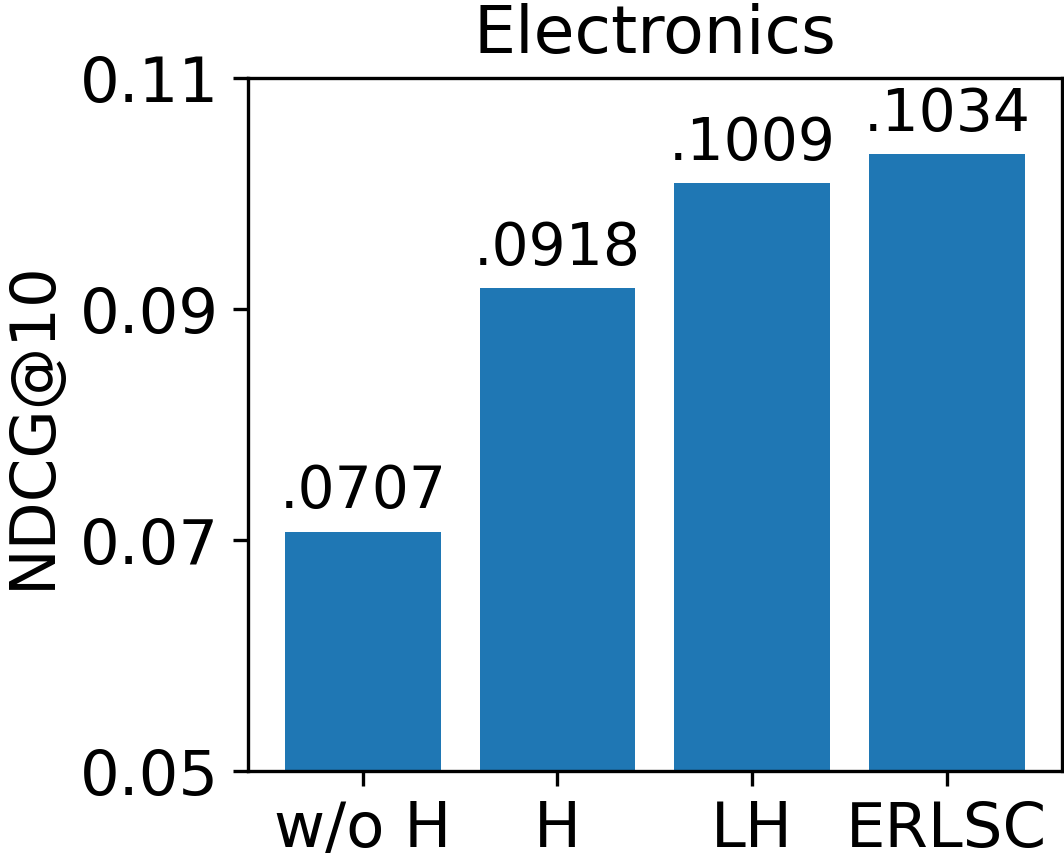
\includegraphics[width=\textwidth]{sections/5_ERLSC/figures/ablation/Electronics_bar.png}
    \end{subfigure}
    \hfill
    \begin{subfigure}{0.3\textwidth}
    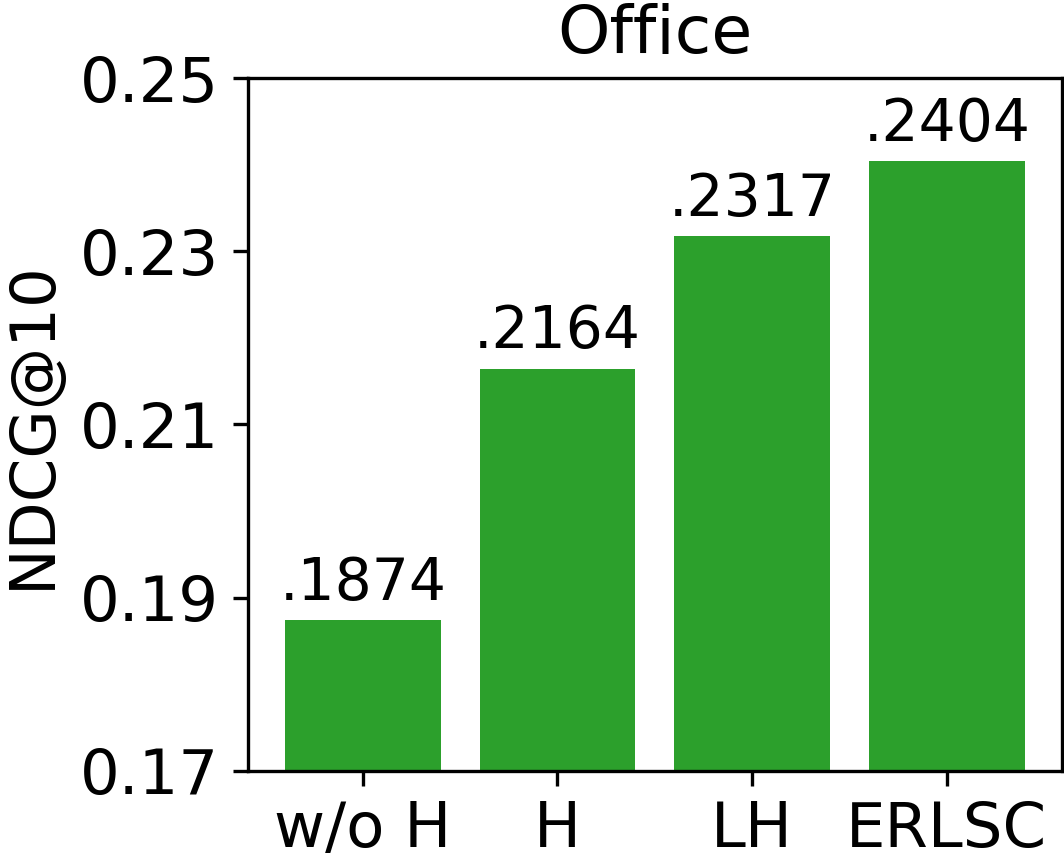
\includegraphics[width=\textwidth]{sections/5_ERLSC/figures/ablation/Office_bar.png}
    \end{subfigure}
    \hfill
    \begin{subfigure}{0.3\textwidth}
    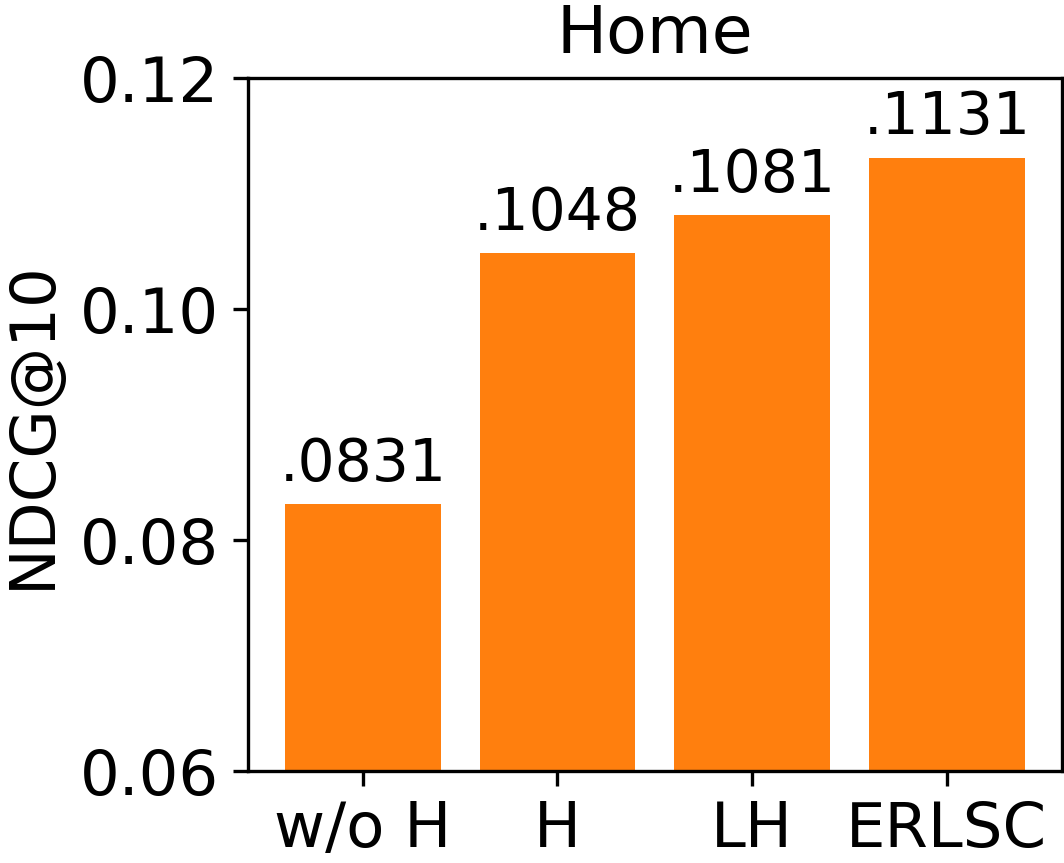
\includegraphics[width=\textwidth]
    {sections/5_ERLSC/figures/ablation/Home_bar.png}
    \end{subfigure}\
    \
        \caption{Performance of ERLSC compared to its variants.}\label{fig:ablation}
\end{figure}

\subsection{Performance under Different Signals}
We evaluate the performance of ERLSC under only one of the four different types of co-occurrence signals provided in the dataset, including \textit{BT} (\textit{bought-together}), \textit{CW} (\textit{compared-with}), \textit{AB} (\textit{also-bought}), and \textit{AV} (\textit{also-viewed}). For each signal type, we construct item–item hyperedges solely based on the corresponding relation and report the results in Table~\ref{tab_erlsc:ablation_2}.
For each signal, we compare the following variants. (i) \textit{BT/CW/AB/AV} only: the LGHC layer is replaced by a naive hypergraph convolution layer. (ii) \{S,C\}$_{max}$: hyperedge weights are initialized as $w_\epsilon = \frac{\max\left(y^{\text{sub}}_\epsilon,\, y^{\text{com}}_\epsilon\right)}{|\mathcal{P}(\mathcal{N}_\epsilon)|}$ which emphasizes whether substitution or complementarity is more prevalent. (iii) S\&C : the full ERLSC\ with a single relation type available. From the results, we observe that incorporating LLM-based relation information consistently improves recommendation performance across all relation types and datasets. Compared with the variants without LGHC, both \{S,C\}$_{max}$ and S\&C achieve noticeable gains, demonstrating the effectiveness of leveraging LLM-inferred substitute and complement signals. Moreover, S\&C used in ERLSC outperforms \{S,C\}$_{max}$ in most cases, indicating that jointly considering substitutes and complements yields more reliable hyperedge weights.




\begin{table}[]
\
\resizebox{0.6\textwidth}{!}{
\begin{tabular}{l|cc|cc|cc}
\hline
\multicolumn{1}{c|}{Dataset} & \multicolumn{2}{c|}{Electronics}    & \multicolumn{2}{c|}{Office}       & \multicolumn{2}{c}{Home}     \\ \hline
Metric                       & R@10             & N@10             & R@10             & N@10             & R@10             & N@10             \\ \hline
\textit{BT} only                   & 0.0921          & 0.0656          & 0.2629          & 0.2170          & 0.1216          & 0.0793          \\
+ \{S,C\}$_{max}$                      & 0.0952          & 0.0719          & 0.2672          & 0.2181          & 0.1199          & 0.0929          \\
+ S\&C                  & 0.1066          & 0.0826          & 0.2684          & 0.2215          &0.1226          & 0.1075          \\ \hline
\textit{CW} only                   & 0.0865          & 0.0710         & 0.2525          & 0.2112          & 0.1118          & 0.0860          \\
+ \{S,C\}$_{max}$                      & 0.0893          & 0.0776          & 0.2555          & 0.2162          & 0.1175          & 0.0943          \\
+ S\&C                       & 0.0979         & 0.0782          & 0.2604          & 0.2189          & 0.1226         & 0.1012          \\ \hline
\textit{AB} only                   & 0.0940          & 0.0765          & 0.2468          & 0.1936          & 0.1182          & 0.0766          \\
+ \{S,C\}$_{max}$                       & 0.0971          & 0.0770          & 0.2450          & 0.2030          & 0.1169          & 0.0889          \\
+ S\&C                        & 0.1066          & 0.0834          & 0.2527          & 0.2062          & 0.1226          & 0.1063         \\ \hline
\textit{AV} only                   & 0.0998          & 0.0858          & 0.2738          & 0.2273          & 0.1189          & 0.0666          \\
+ \{S,C\}$_{max}$                       & 0.1089          & 0.0845          & 0.2747          & 0.2296          & 0.1216          & 0.1078          \\
+ S\&C                       & 0.1140          & 0.0878          & 0.2790          & 0.2328          & 0.1274          & 0.1076          \\ \hline
\end{tabular}
}\caption{Performance of ERLSC on each single relation type.}\label{tab_erlsc:ablation_2}
\
\end{table}


\section{Chapter Summary}

In this chapter, we investigate how to leverage LLMs to assess substitute and complementary relations and to adaptively determine hyperedge weights through the proposed LGHC layer. Experimental results on real-world datasets demonstrate the effectiveness of incorporating LLM-encoded world knowledge on substitution and complementarity into recommendation models.
However, ERLSC still follows a single-model learning paradigm, where the final recommendation performance depends on a single trained model, even when enhanced by LLM-derived relational signals. In the next chapter, we move beyond this paradigm and introduce an LLM-based agent framework that coordinates multiple recommendation tools and performs explicit relational reasoning at inference time.
